
%\documentclass[12pt]{amsart}
%\usepackage{geometry} % see geometry.pdf on how to lay out the page. There's lots.
%\geometry{a4paper} % or letter or a5paper or ... etc
% \geometry{landscape} % rotated page geometry

\documentclass[11pt,letter]{article}

%\usepackage[latin1]{inputenc}
\usepackage{epsfig}
\usepackage{amsmath}
\usepackage{mdframed}
%\usepackage{amsfonts}
\usepackage{amssymb}
\usepackage{listings}
\usepackage{booktabs}
\usepackage{setspace}
\usepackage[colorlinks,citecolor=blue]{hyperref}
\usepackage{xcolor}
\usepackage[sort&compress,numbers]{natbib}
%\usepackage{natbibspacing}

\setlength{\oddsidemargin}{.46cm}
\setlength{\evensidemargin}{-0.46cm}
\setlength{\evensidemargin}{0.0cm}
\setlength{\textwidth}{15.5cm}
\setlength{\parskip}{1.0ex plus 0.6ex minus 0.6ex}
\setlength{\parindent}{1.0em} 
\setlength{\textheight}{22.5cm}
\setlength{\topmargin}{-2cm}
\setlength{\footskip}{2cm}
\setlength{\parindent}{0.0cm}

\def\aj{Astron. J.}
\def\apj{Astrophys. J.}
\def\apjl{Astrophys. J. Lett.}
\def\apjs{Astrophys. J. Supp. Ser. }
\def\aa{Astron. Astrophys. }
\def\aap{Astron. Astrophys. }
\def\araa{Ann.\ Rev. Astron. Astroph. }
\def\physrep{Phys. Rep. }
\def\mnras{Mon. Not. Roy. Astron. Soc. }
\def\mmsun{M_\odot}
\def\prl{Phys. Rev. Lett.}
\def\prd{Phys. Rev. D.}
\def\azh{Soviet Astron.}
\def\apss{Astrophys. Space Sci.}
\def\cqg{Class. Quantum Grav.}

\usepackage{mdframed}
\usepackage{mathpazo}
\DeclareMathOperator{\diff}{d\!}
\newcommand{\modot}{M$_\odot$\hspace*{0.05cm}}
\def\apj{Astrophys. Journal}
\def\apjl{Astrophys. Journal Letters}
\def\aap{Astron. Astrophys.}

\setlength{\parskip}{.2cm}

\newcommand{\pd}[2]{\frac{\partial #1}{\partial #2}} 
\newcommand{\pdtwo}[3]{\frac{\partial #1}{\partial #2 \partial #3}} 
\newcommand{\pdtri}[4]{\frac{\partial #1}{\partial #2 \partial #3 \partial #4}} 
\newcommand{\grad}{\vec{\nabla}}
\newcommand{\ddiv}{\vec{\nabla}\cdot}
\newcommand{\intl}{\int\limits}
\newcommand{\msun}{M$_\odot$\ }
\newcommand{\mo}{\mathrm{M}_\odot }
\newcommand{\code}[1]{{\tt #1}}
\newcommand{\todo}[1]{{$\blacksquare$~\textbf{\color{blue}[TODO: #1]}}~$\blacksquare$}
\newcommand{\warn}[1]{{$\blacksquare$~\textbf{\color{red}[WARNING: #1]}}~$\blacksquare$}

% See the ``Article customise'' template for come common customisations

\title{Density dependent surface energy and pressure of nuclei in medium}
\author{Ermal Rrapaj}
\date{} % delete this line to display the current date
\begin{document}
\maketitle


\section{Woods-Saxon density profile for nucleus in medium}
Our description of the Wigner seitz cell:
\begin{center}
 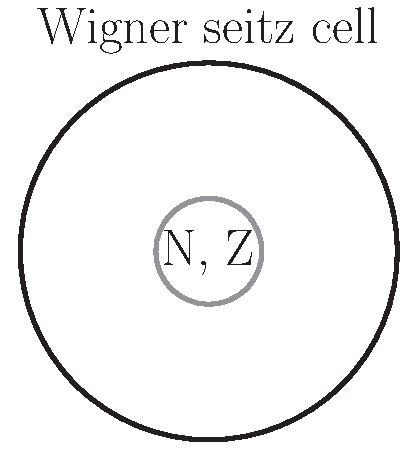
\includegraphics[scale=0.4]{WSC.pdf}
\end{center}

Woods-Saxon model:

The desnity profile of the Wigner seitz cell is decomposed in terms of the Woods - Saxon function for the high density region (nucleus) and the low denisty 
region (nuclear medium outside):
\begin{center}
 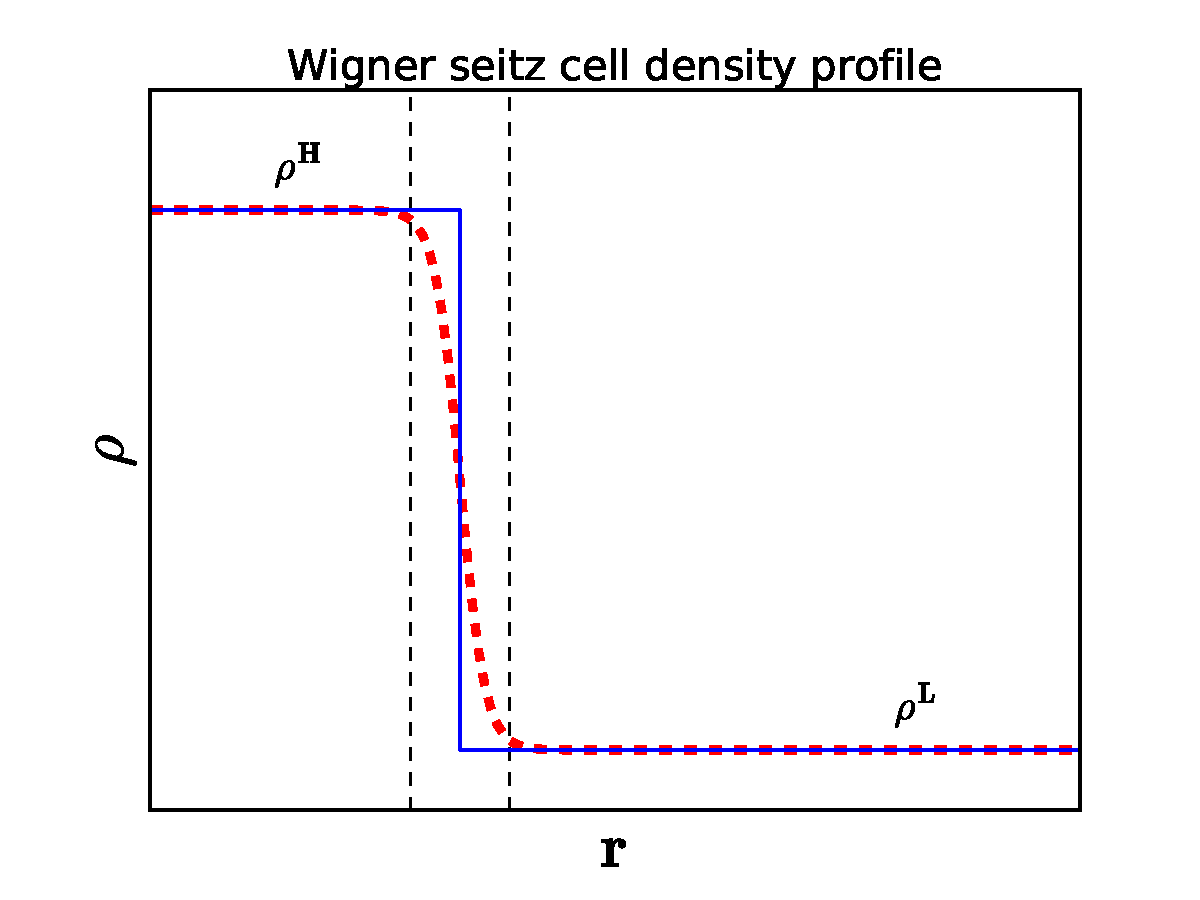
\includegraphics[scale=0.6]{WSCprofile.pdf}
\end{center}
\begin{equation}
 \begin{split}
  n(r) = & n_{Nuc}(r)+n_{gas}(r) \\
  =&\frac{n^{H}}{1+\exp[(r-R^{WS})/a_{WS}]} + \frac{n^{L}}{1+\exp[-(r-R^{WS})/a_{WS}]} 
 \end{split}
\end{equation}
where,
\begin{equation}
 \begin{split}
  a_{WS} =& \alpha + \beta (\delta^{H}_{np})^2,\ \alpha \approx 0.53\ \text{fm}, \beta_n \approx 1.14\ \text{fm},\ \beta_p \approx 0.35\ \text{fm} \\
  R^{WS} =& R_{i}[1-\frac{\pi^2}{3}(\frac{a}{R_i})^2]\\
  R_i =& (\frac{3 V_i}{4\pi})^{1/3}\\
  =& (\frac{3 A_i}{4\pi n^H})^{1/3}
 \end{split}
\end{equation}
Assuming $a \ll R_i \rightarrow R^{WS}\approx R_i$. 

In our model, we assume two homogeneous phases of matter at different densities with a sharp transition from one to the other.
This is represented by the step function in the figure.
In order to make the 2 descriptions match, our description needs to include a surface contribution:
\begin{equation}
 \begin{split}
  E^H(R^{WS}-4a,R)+E^L(R,R^{WS}+4a)+E^{S}=E^{WS}(R^{WS}-4a,R^{WS}+4a),\ E^{S} = 4\pi (R^{WS})^2 \sigma
 \end{split}
\end{equation}
where, $E^H,\ E^L$ are the energies of homogeneous matter at $\rho^H,\ \rho^L$ respectively. $E^{WS}$ is the 
energy of non-constant matter.

The skyrme energy density:
\begin{equation}
 \begin{split}
  E/V &= \sum_{t=n,p}\frac{\hbar^2}{2M_q}\tau_q+\frac{1}{4}t_0\Big[(2+x_0)n^2-(1+2x_0)\sum_{q=n,p} n^2_q\Big]\\
  &+\frac{1}{8}\Big[ a (n \tau+\frac{3}{4}(\triangledown n)^2)+2b\sum_{q=n,p}(n_q \tau_q+\frac{3}{4}(\triangledown n_q)^2)\Big]\\
  &+\frac{1}{24}t_3n^{\alpha}\Big[(2+x_3)n^2-(1+2x_3)\sum_{q=n,p}n_q^2\Big]\\
  &=(E/V)_{h}+\frac{3}{32}\Big[ a (\triangledown n)^2+2b\sum_{q=n,p}(\triangledown n_q)^2)\Big]\\
 \end{split}
\end{equation}
Again assuming $a\ll R^{WS}$:
\begin{equation}
 \begin{split}
  4\pi (R^{WS})^2\ \sigma \approx& [4\pi (R^{WS})^2\times 8a_{WS}] \times   \frac{3}{32}\Big[ a (\triangledown n)^2+2b\sum_{q=n,p}(\triangledown n_q)^2)\Big] \leftrightarrow \\
\sigma =& \frac{3a_{WS}}{4} \Big[a (\frac{dn}{dr})^2 +2 b \big( (\frac{dn_n}{dr})^2+(\frac{dn_p}{dr})^2\big) \Big]\bigg |_{R^{WS}}\\ 
 \end{split}
\end{equation}
Given the functional form of the density profile: $(\frac{dn}{dr})^2 \bigg|_{r=R^{WS}} = \frac{(n_H-n_L)^2}{16\ {a_{WS}}^2}$.
And, $a_{WS}=a_B \approx a_n$:
\begin{equation}
 \begin{split}
  \sigma =& \frac{3}{64} \frac{(n_H-n_L)^2}{a_{WS}}  \big[a\  +2 b ( 1+\frac{a_{WS}^2}{a_p^2})\big]\leftrightarrow \\
 \end{split}
\end{equation}

\begin{mdframed}
\begin{equation*}
  \begin{split}
  \sigma=&\frac{3}{64} \frac{(n_H-n_L)^2}{\alpha+\beta_n \ {\delta^H_{np}}^2} \big[a\  +2 b ( 1+\frac{(\alpha+\beta_n \ {\delta^H_{np}}^2)^2}{(\alpha+\beta_p \ {\delta^H_{np}}^2)^2})\big]\\
  a_{WS} =& \alpha + \beta (\delta^{H}_{np})^2,\ \alpha \approx 0.53\ \text{fm}, \beta_n \approx 1.14\ \text{fm},\ \beta_p \approx 0.35\ \text{fm} 
  \end{split}
 \end{equation*}
\end{mdframed}
For ordinary nuclei (no surrounding nuclear medium) the diffuseness parameter is $a_{WS} = 0.55 \pm 0.05 \ \text{fm}$ 
\end{document}
